\chapter{Appendix}

\section{Gallery of Visual Examples}

\subsection{Local Fractal Dimension}

\subsection{Global Fractal Dimension}

\subsection{Euler Characteristic}

\section{Fractal Dimension}
% Dendrograms (maybe)

% to-do
% likely to redo, very messy
\begin{figure}[t]
    \centering
    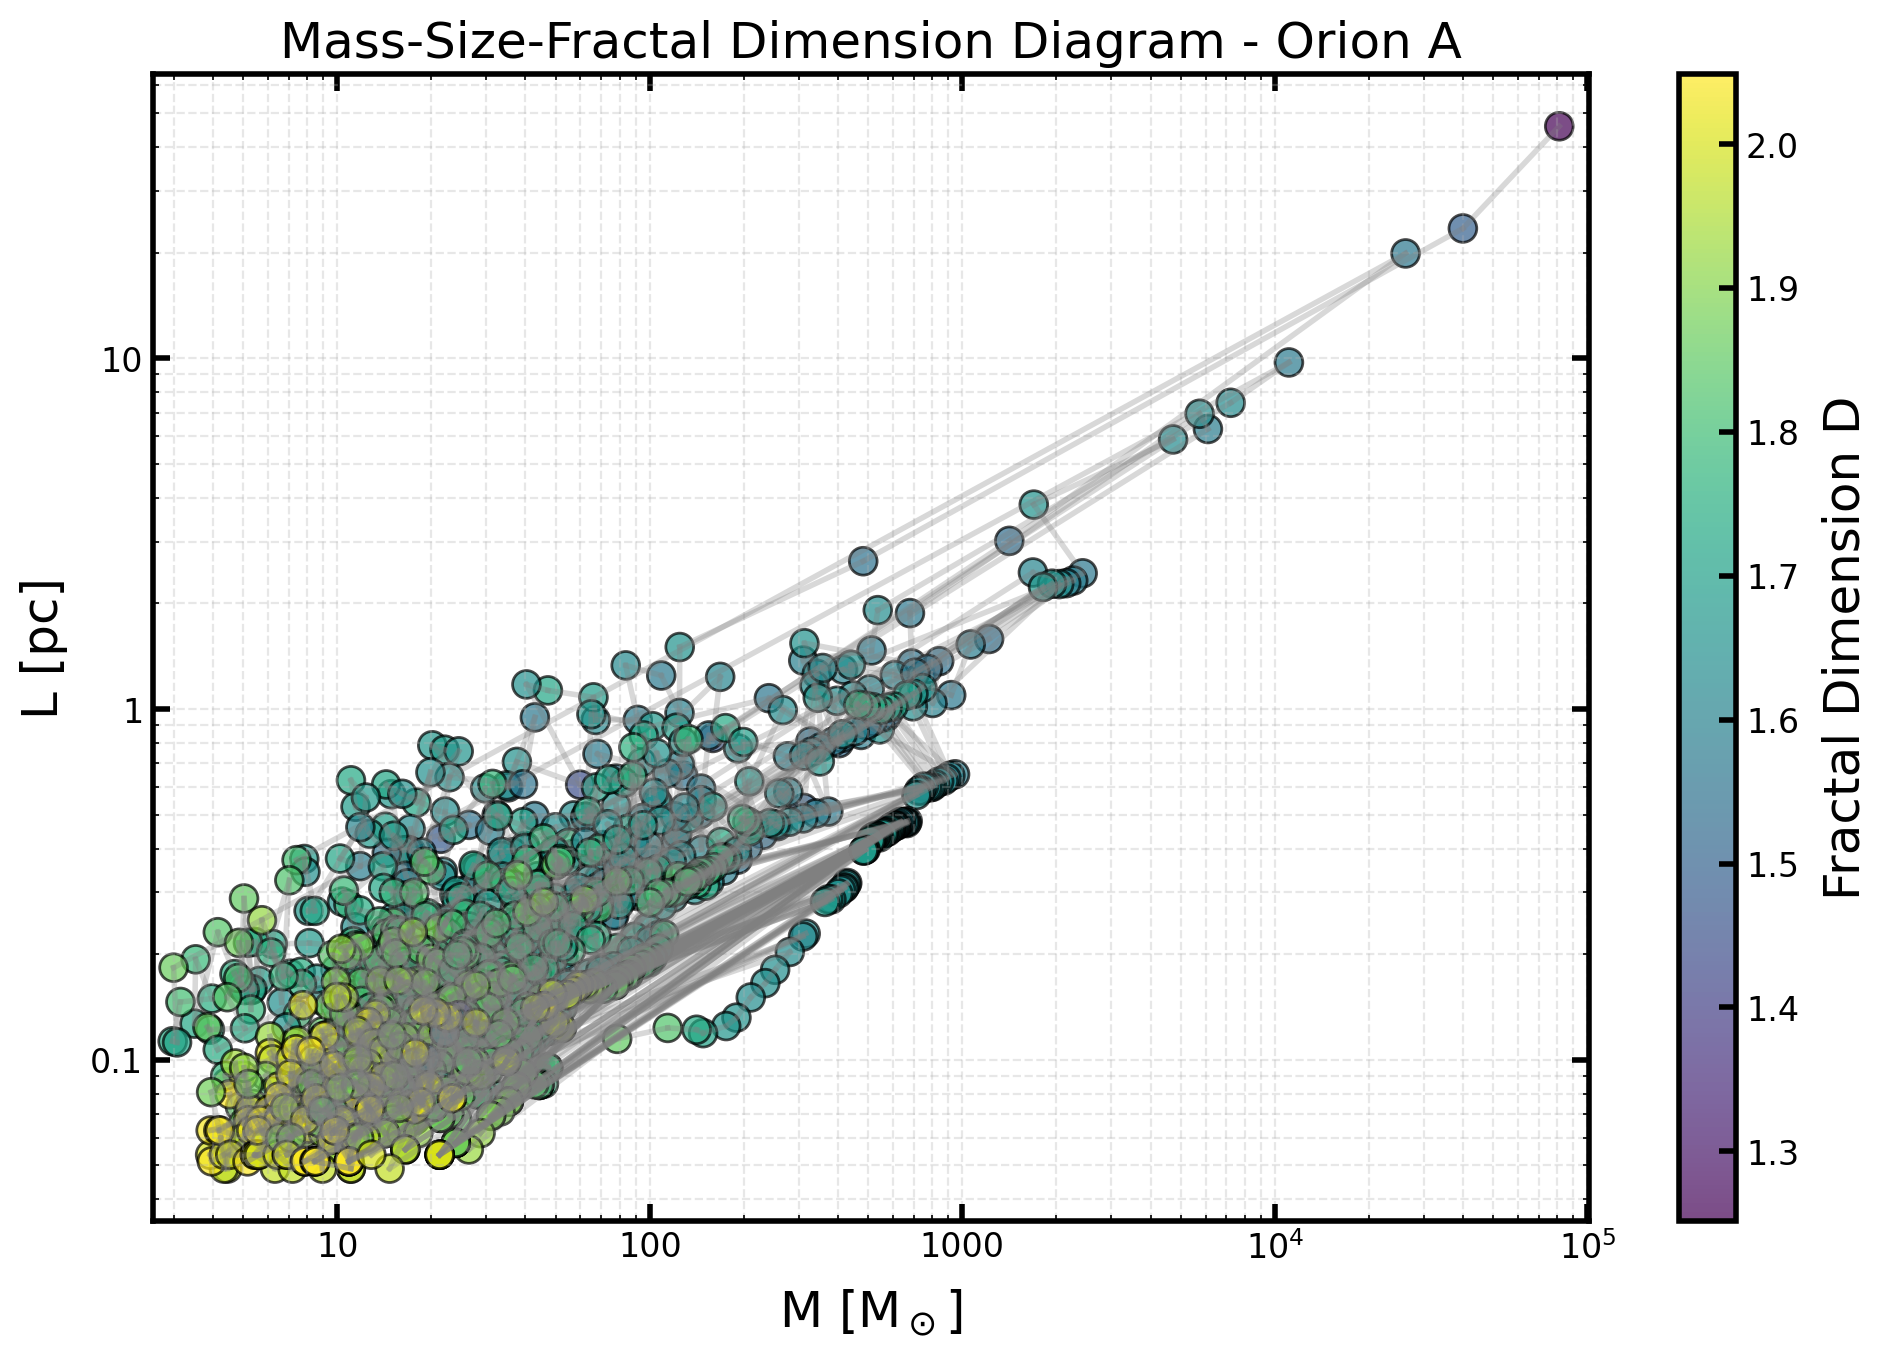
\includegraphics[width=0.5\textwidth]{figures/MSD_Orion_A_with_lines.png}
    \caption{MSD plane for Orion~A with dendrogram connections overplotted. Lines trace parent-child relationships between structures.}
    \label{fig:MSD_orion_A_lines}
\end{figure}

\begin{figure}[t]
    \centering
    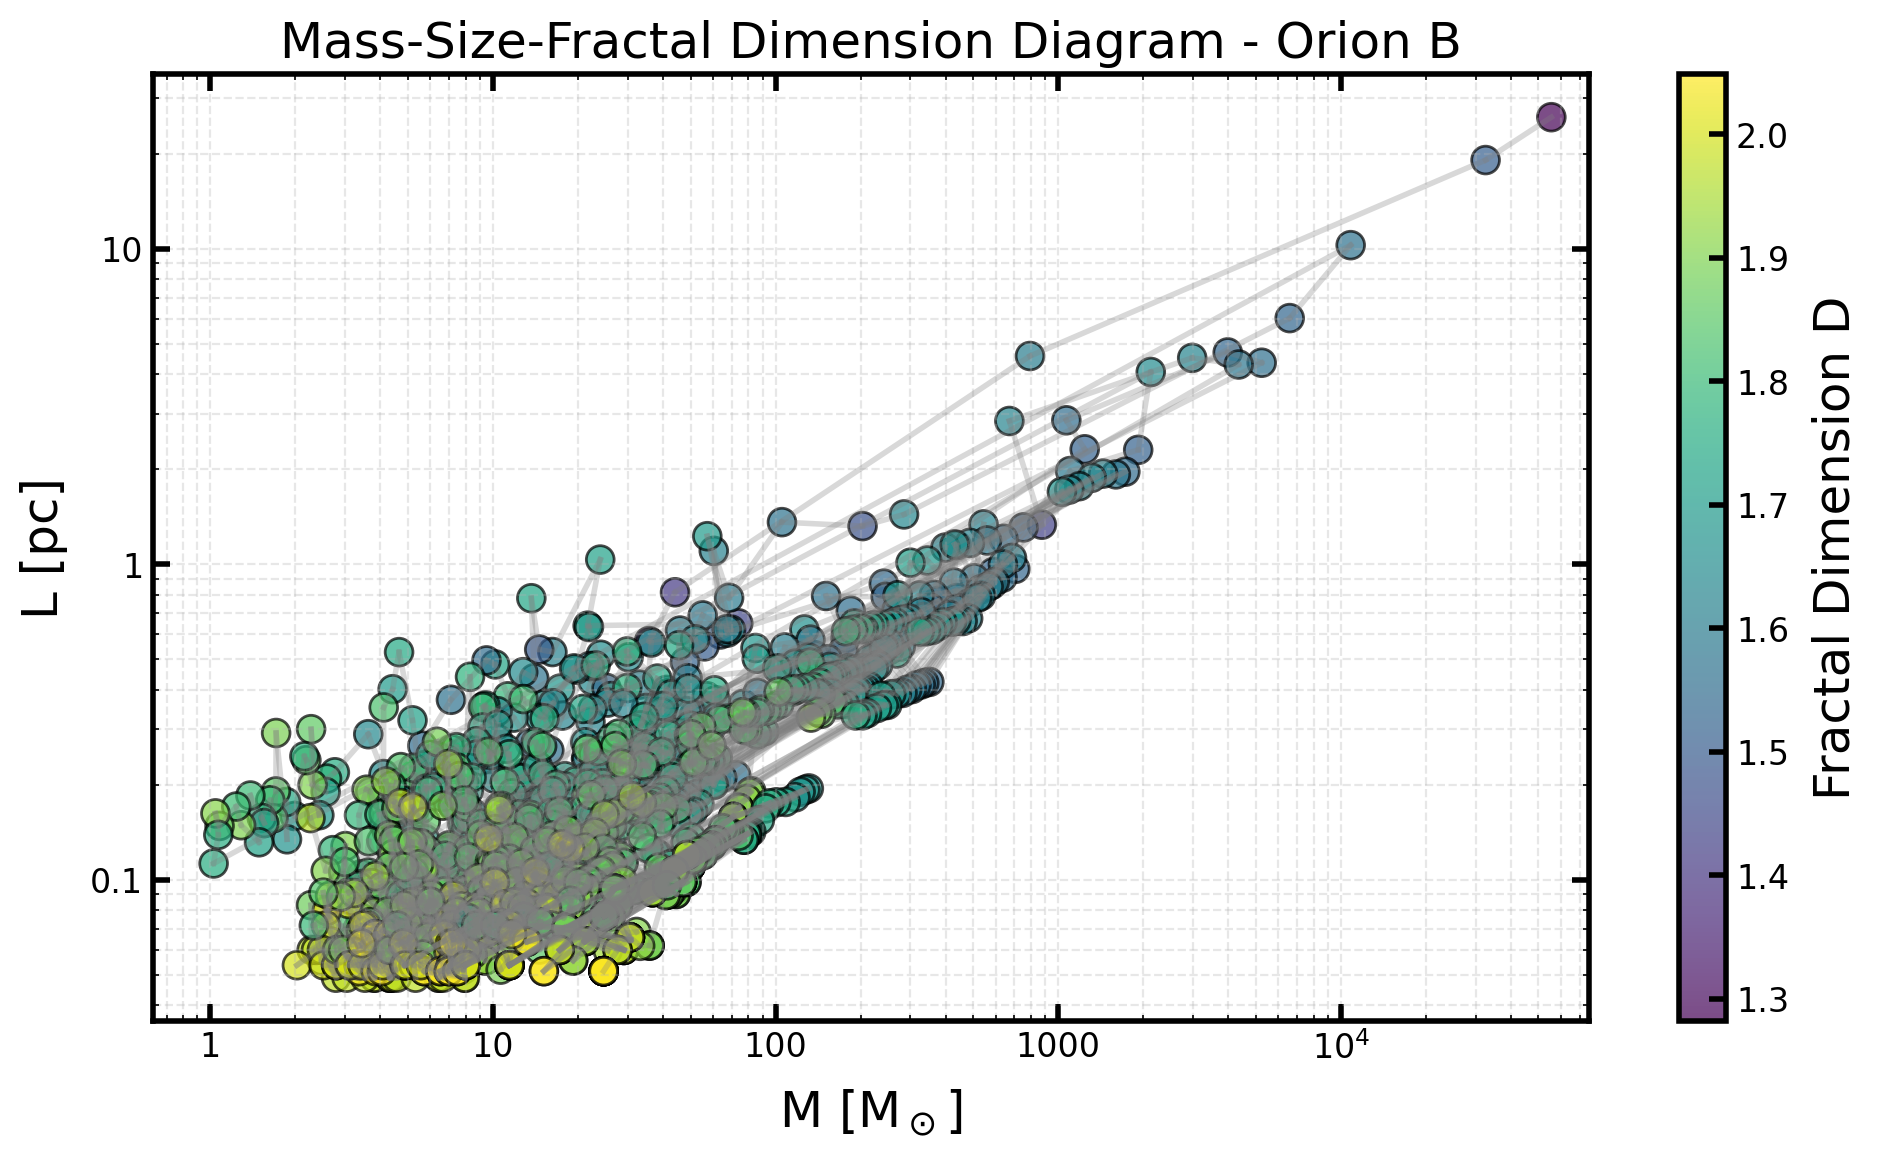
\includegraphics[width=0.5\textwidth]{figures/MSD_Orion_B_with_lines.png}
    \caption{MSD plane for Orion~B with dendrogram connections overplotted.}
    \label{fig:MSD_orion_B_lines}
\end{figure}

\section{YSO Density Maps}

\subsection{Class I/flat-spectrum sources}

\begin{figure}[t]
    \centering
    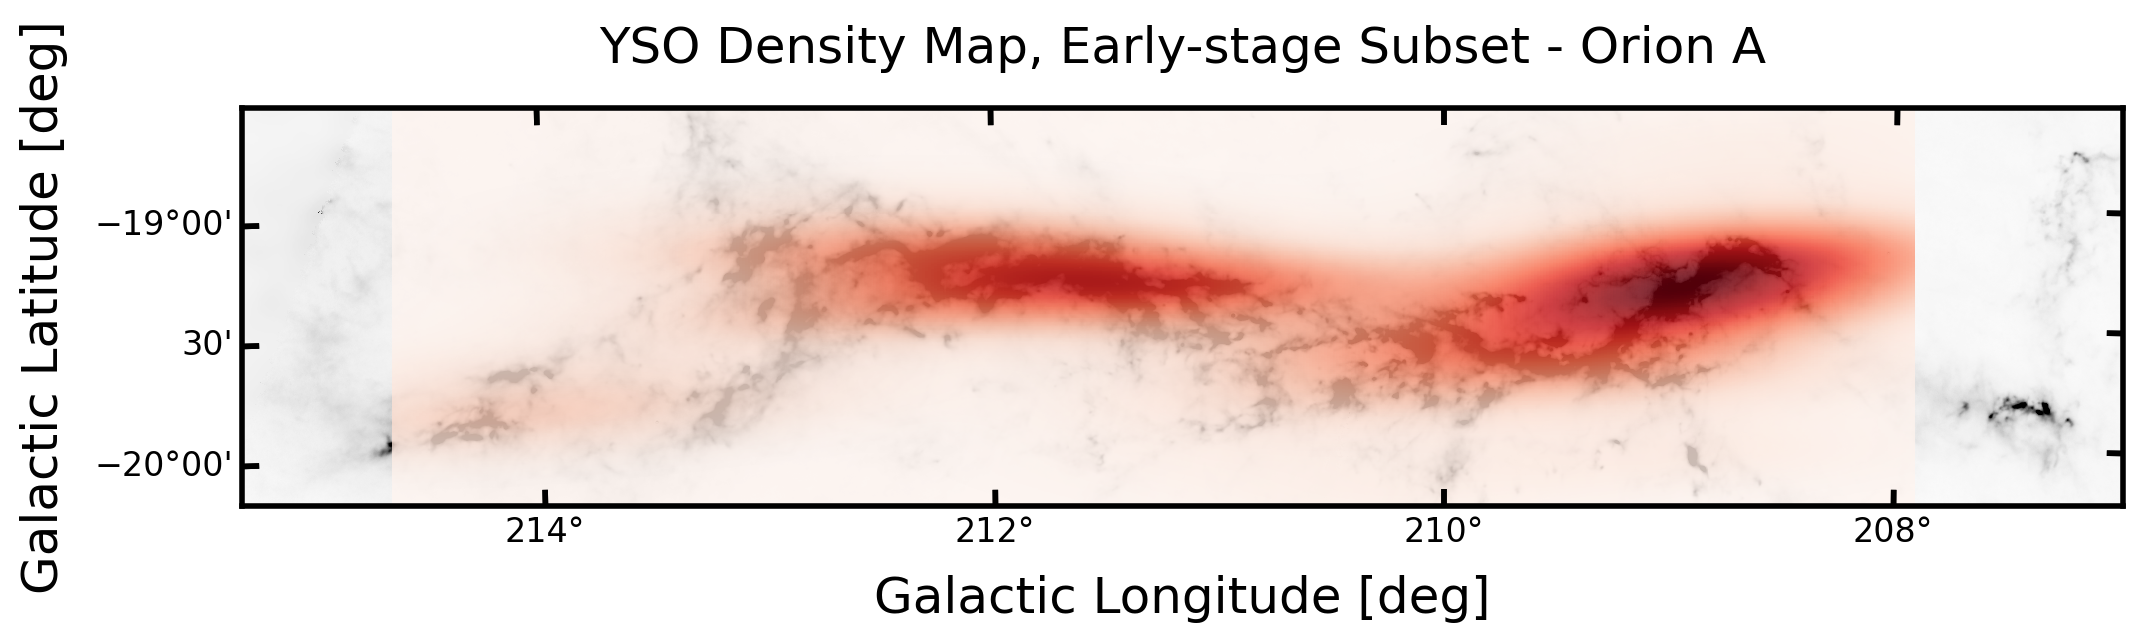
\includegraphics[width=0.75\textwidth]{figures/YSOs_early_stage_density_Orion_A.png}
    \caption{YSO density map for Orion~A, overlaid on the column-density map. The coverage is limited by the extent of the YSO catalog, so some regions are not sampled.}
    \label{fig:YSOs_density_Map_A_early_stages}
\end{figure}

\begin{figure}[t]
    \centering
    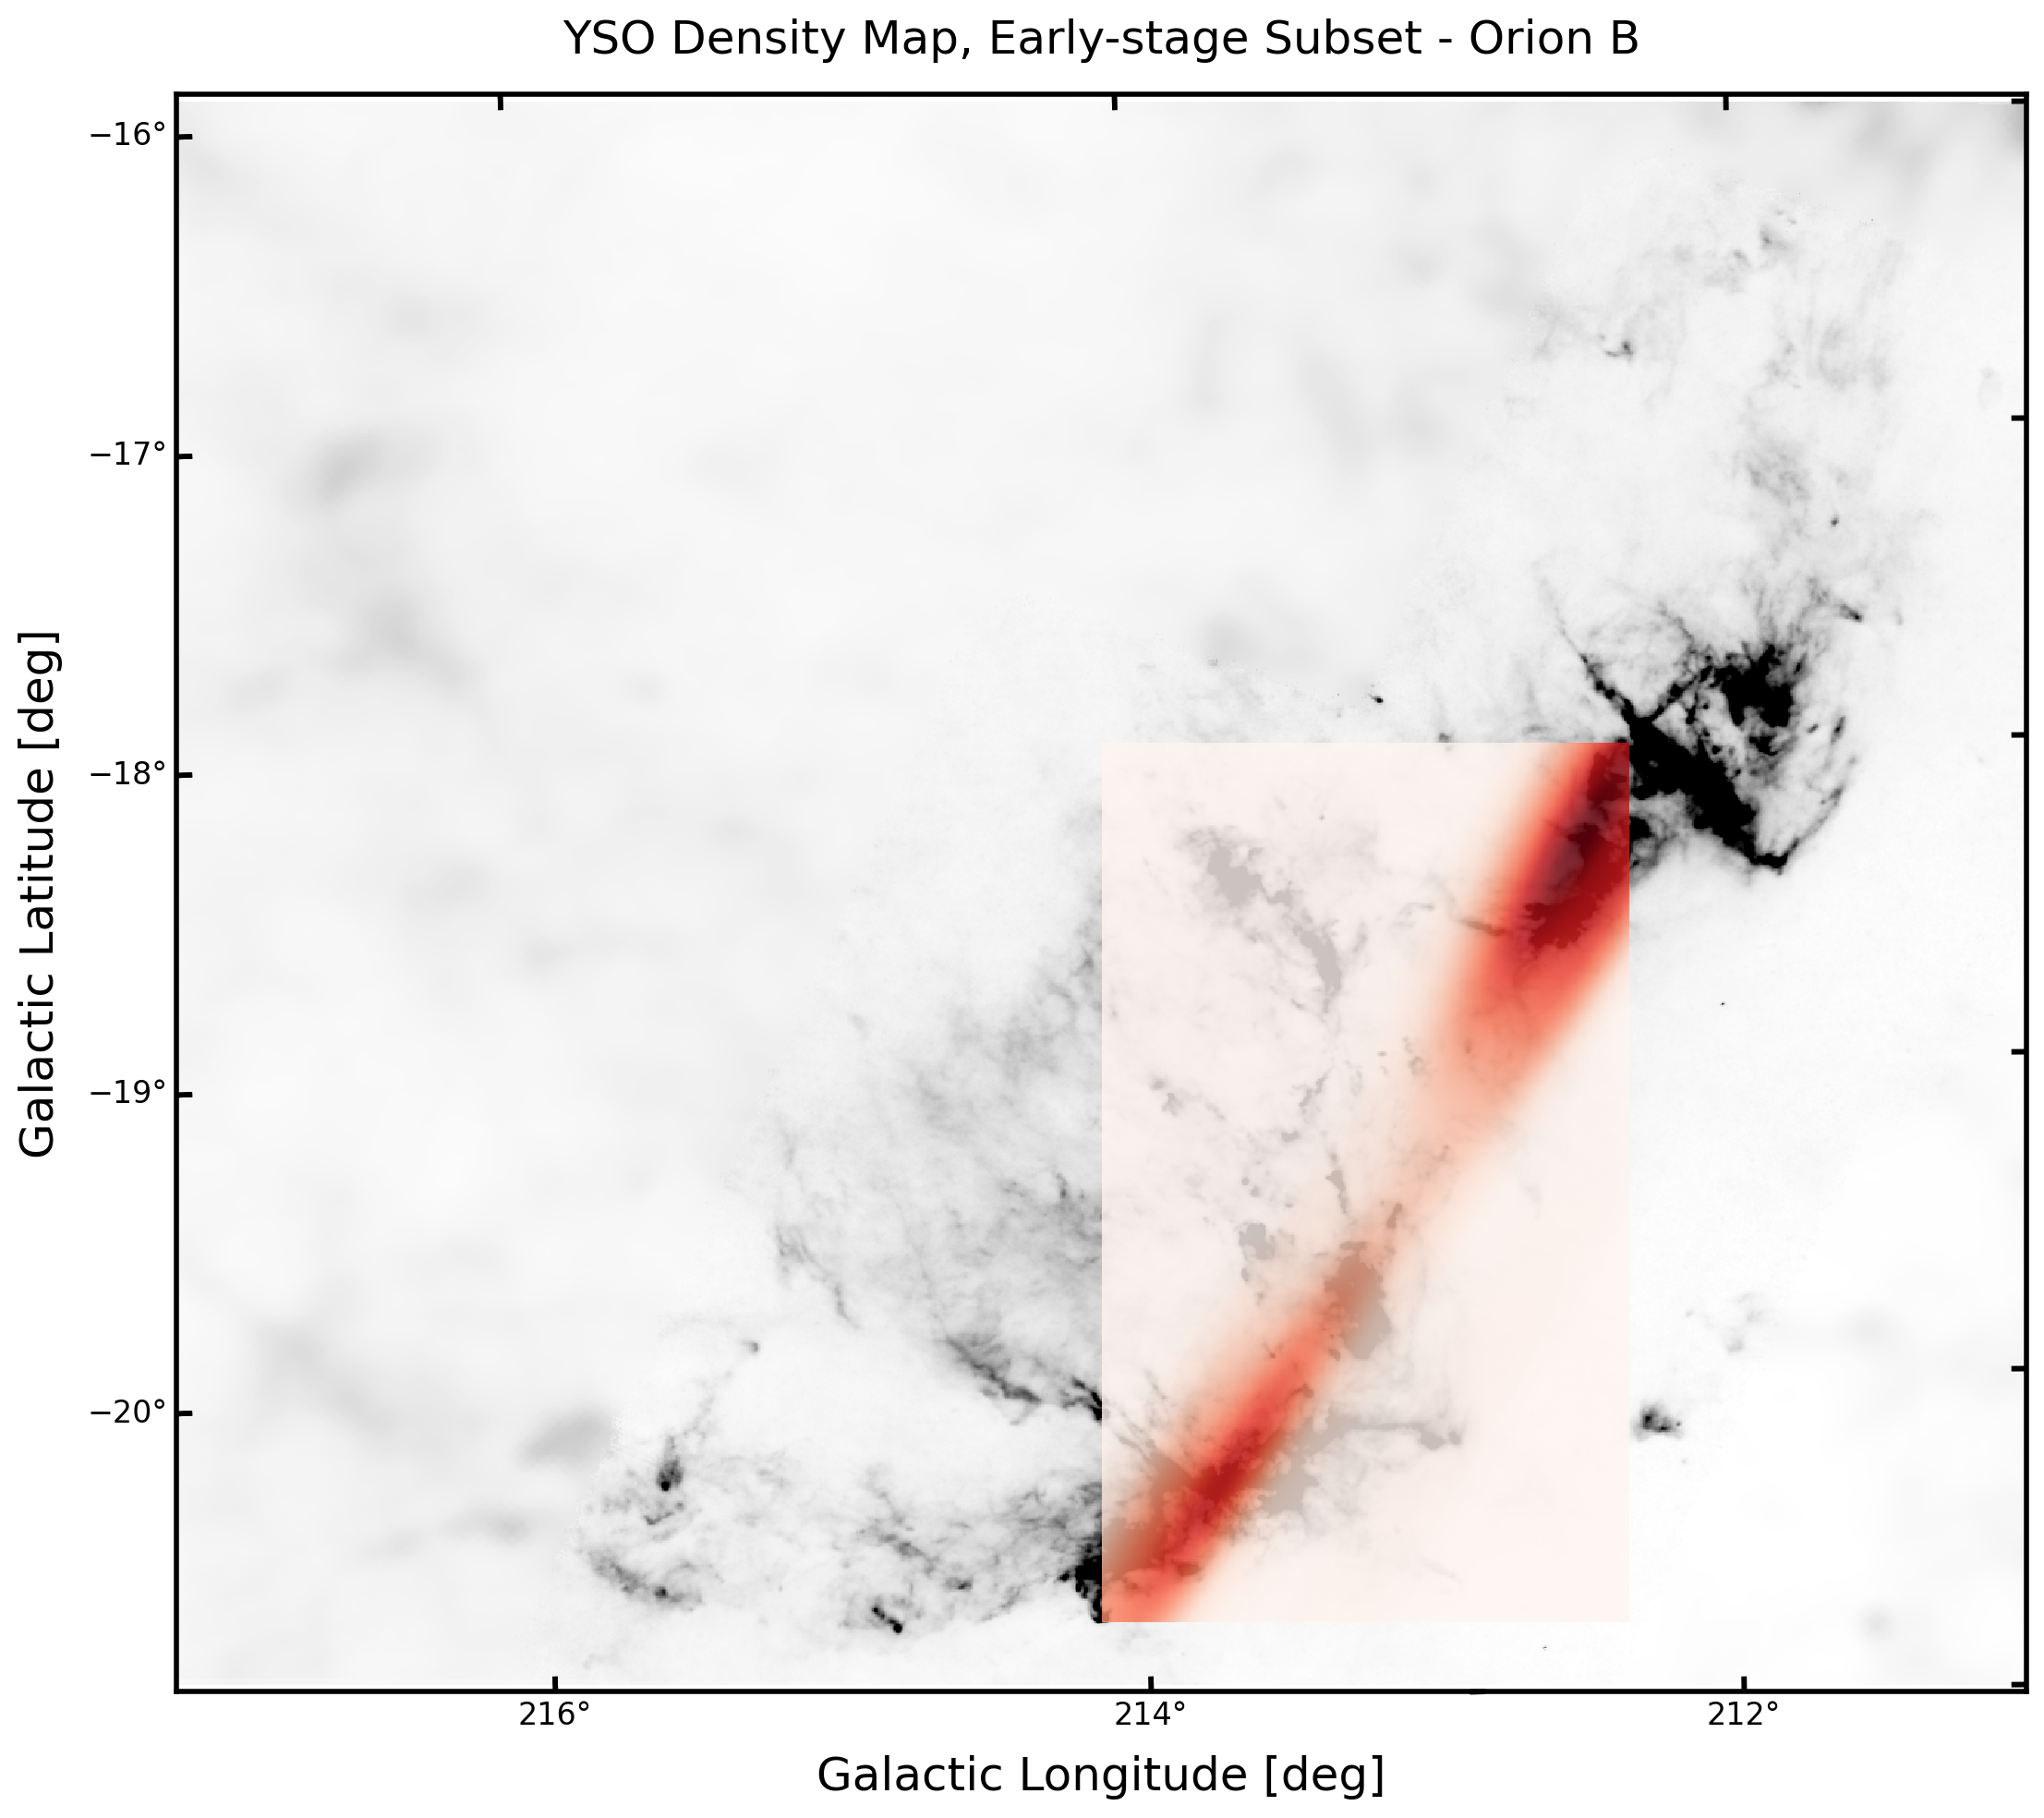
\includegraphics[width=0.75\textwidth]{figures/YSOs_early_stage_density_Orion_B.png}
    \caption{YSO density map for Orion~A, overlaid on the column-density map. The coverage is limited by the extent of the YSO catalog, so some regions are not sampled.}
    \label{fig:YSOs_density_Map_B_early_stages}
\end{figure}

\subsection{Full Sample}

\begin{figure}[t]
    \centering
    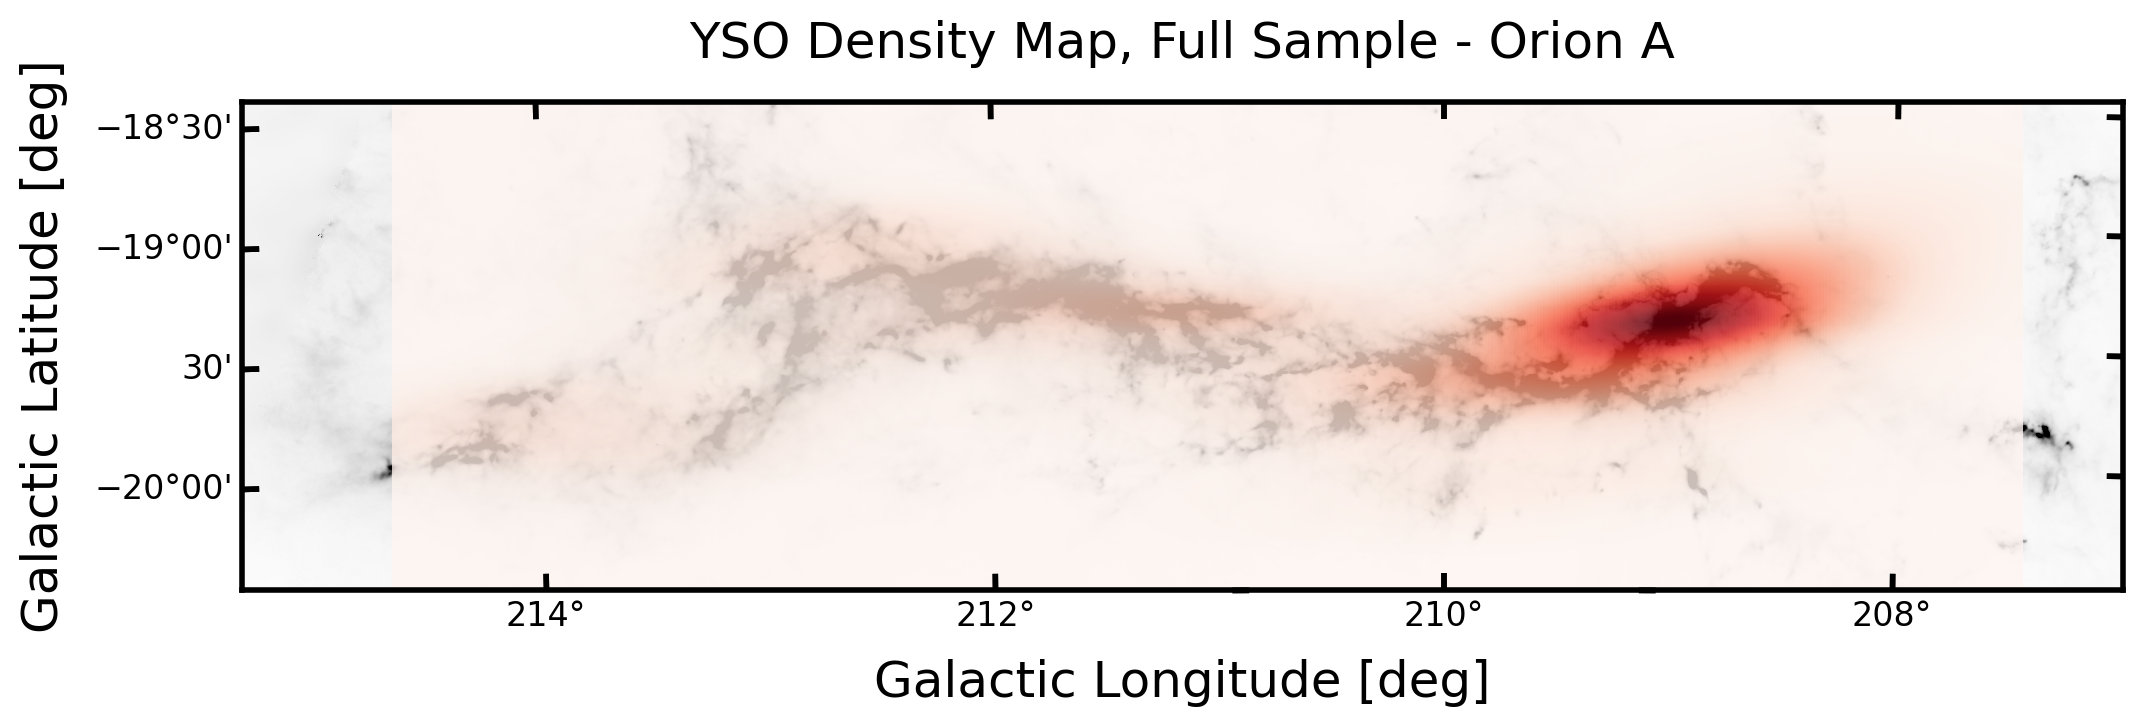
\includegraphics[width=0.75\textwidth]{figures/YSOs_density_Orion_A.png}
    \caption{YSO density map for Orion~A, overlaid on the column-density map. The coverage is limited by the extent of the YSO catalog, so some regions are not sampled.}
    \label{fig:YSOs_density_Map_A}
\end{figure}

\begin{figure}[t]
    \centering
    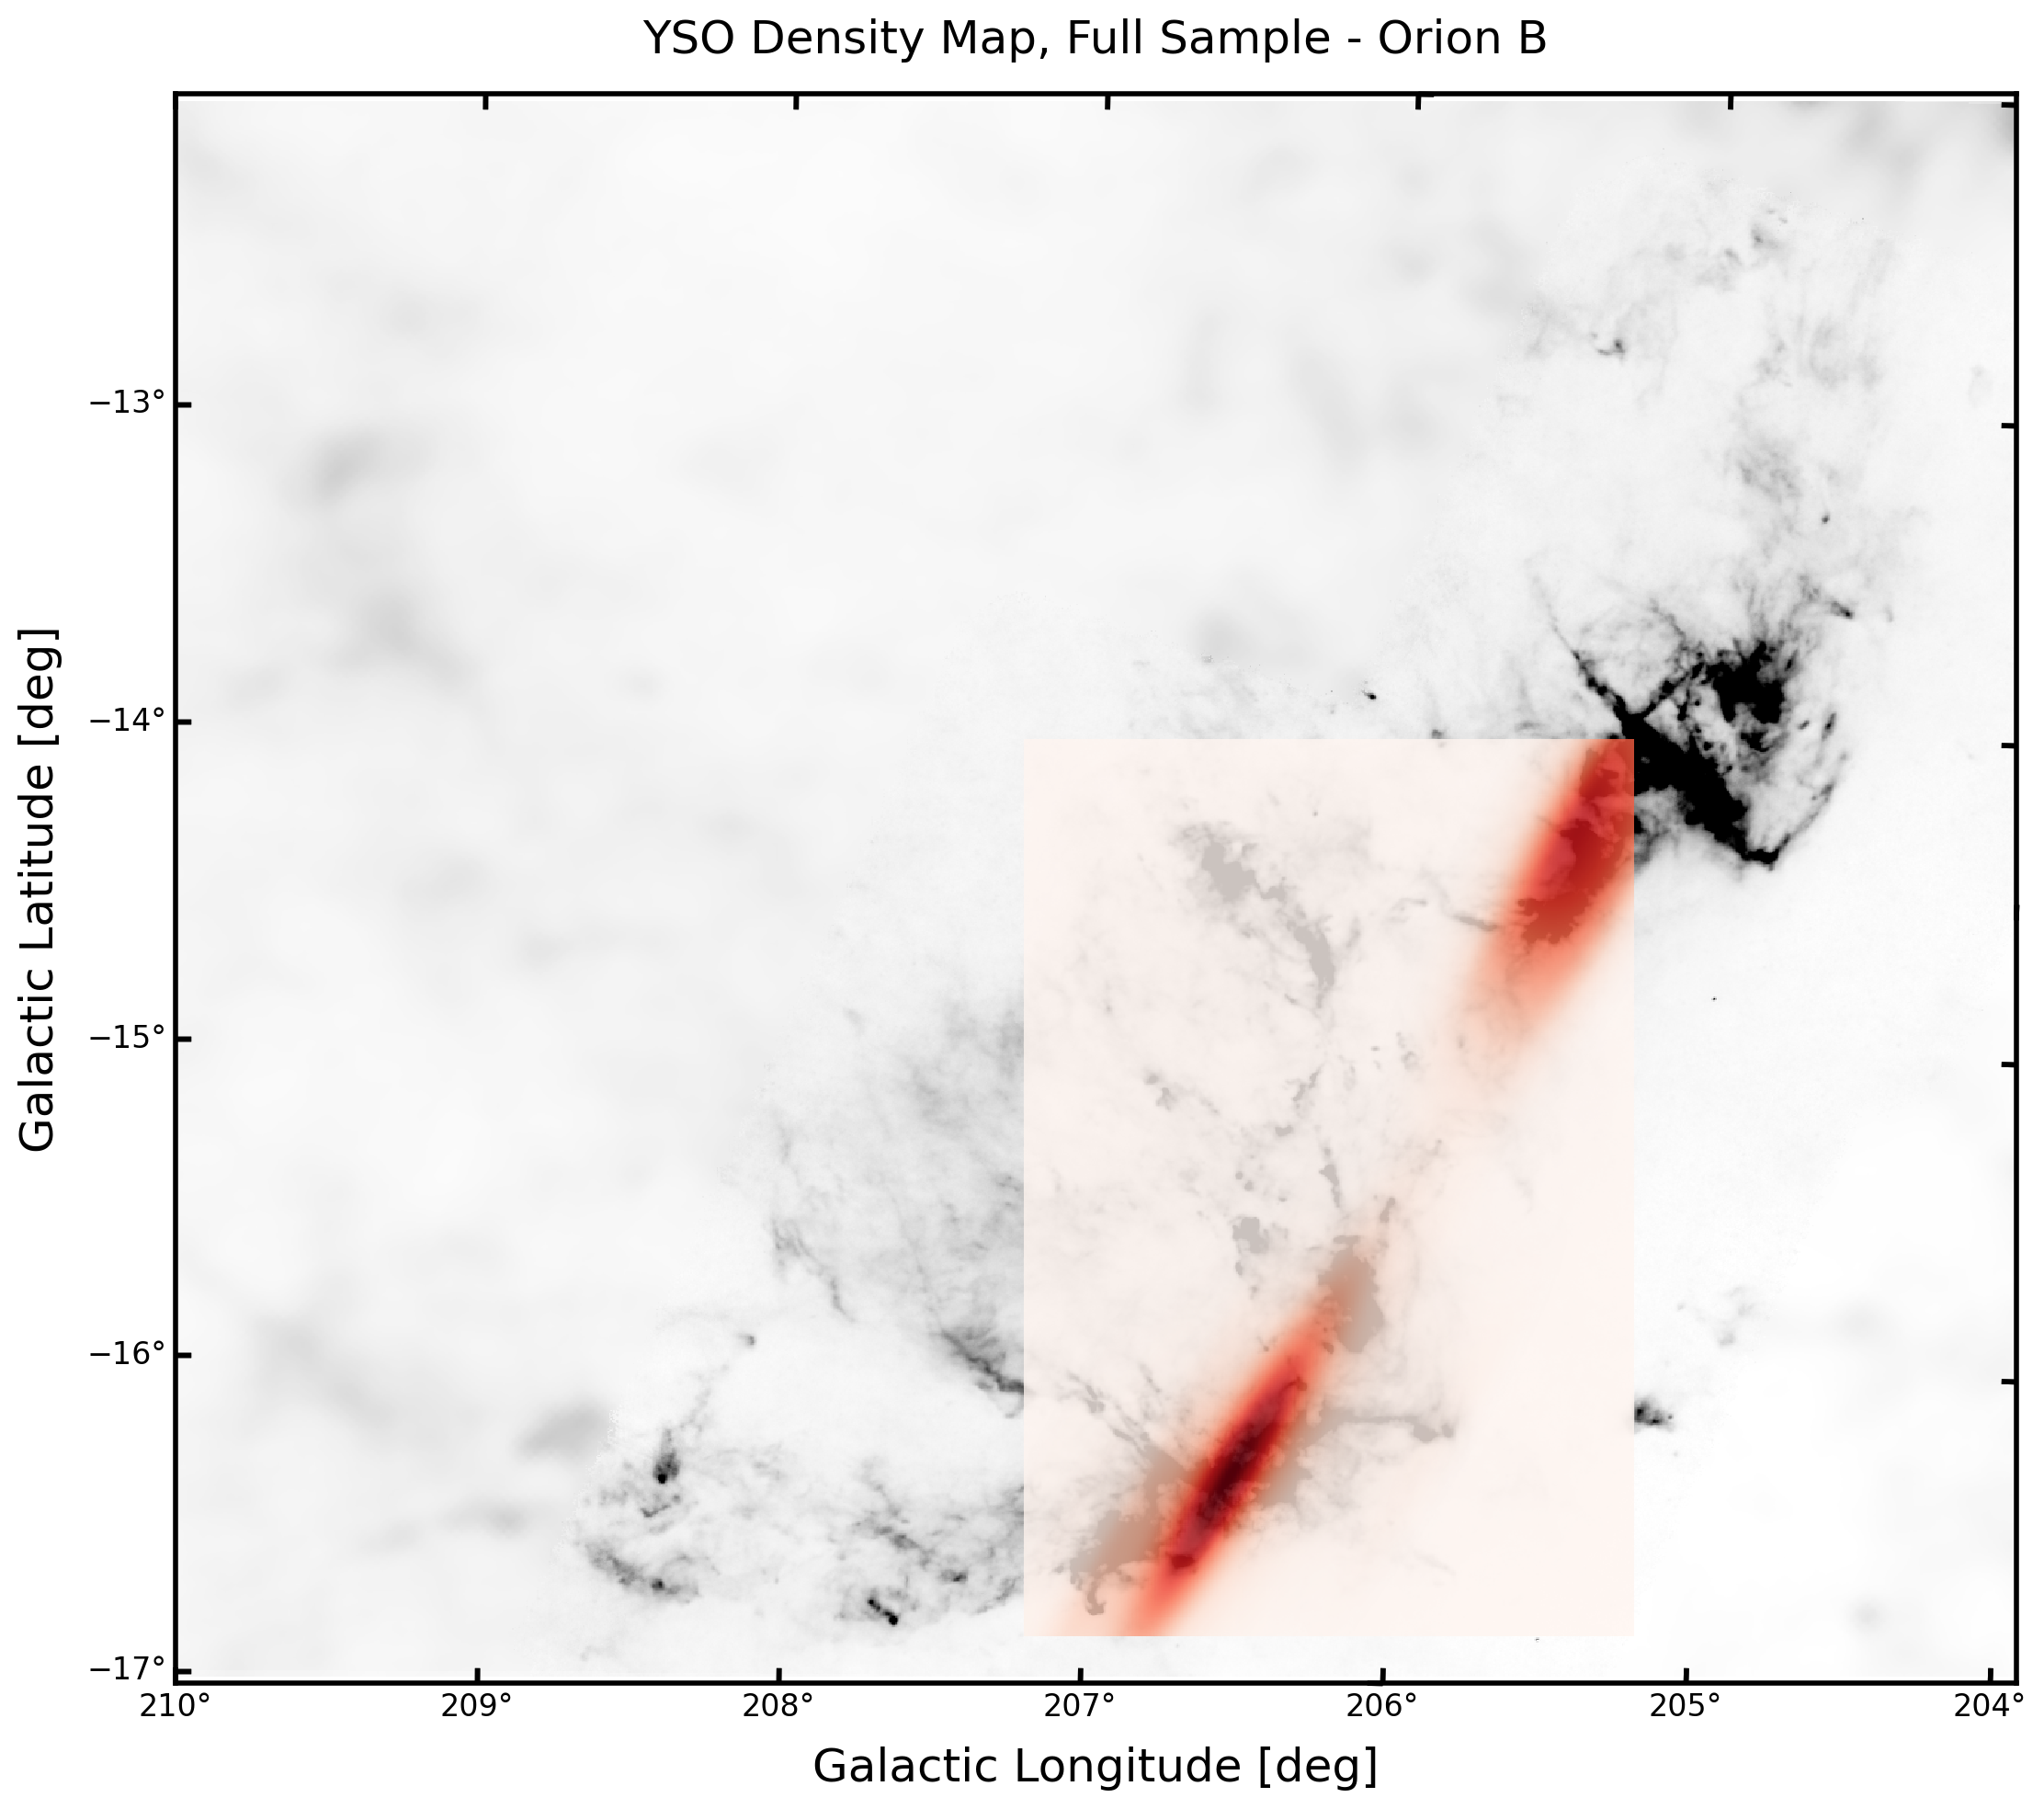
\includegraphics[width=0.75\textwidth]{figures/YSOs_density_Orion_B.png}
    \caption{YSO density map for Orion~A, overlaid on the column-density map. The coverage is limited by the extent of the YSO catalog, so some regions are not sampled.}
    \label{fig:YSOs_density_Map_B}
\end{figure}

\section{Simulations}

\subsection{Global Fractal Dimension}
% simulations global fractal dimension: D = 1 for simple shapes, gets higher the more complex it becomes 
% simulations global fractal dimension: GRF (scale free vs with scale) example
% simulations global fractal dimension: resolution effects

\subsection{Local Fractal Dimension}
% simulations local fractal dimension: resolution effects

\subsection{Uncertainties}

\begin{figure}[t]
    \centering
    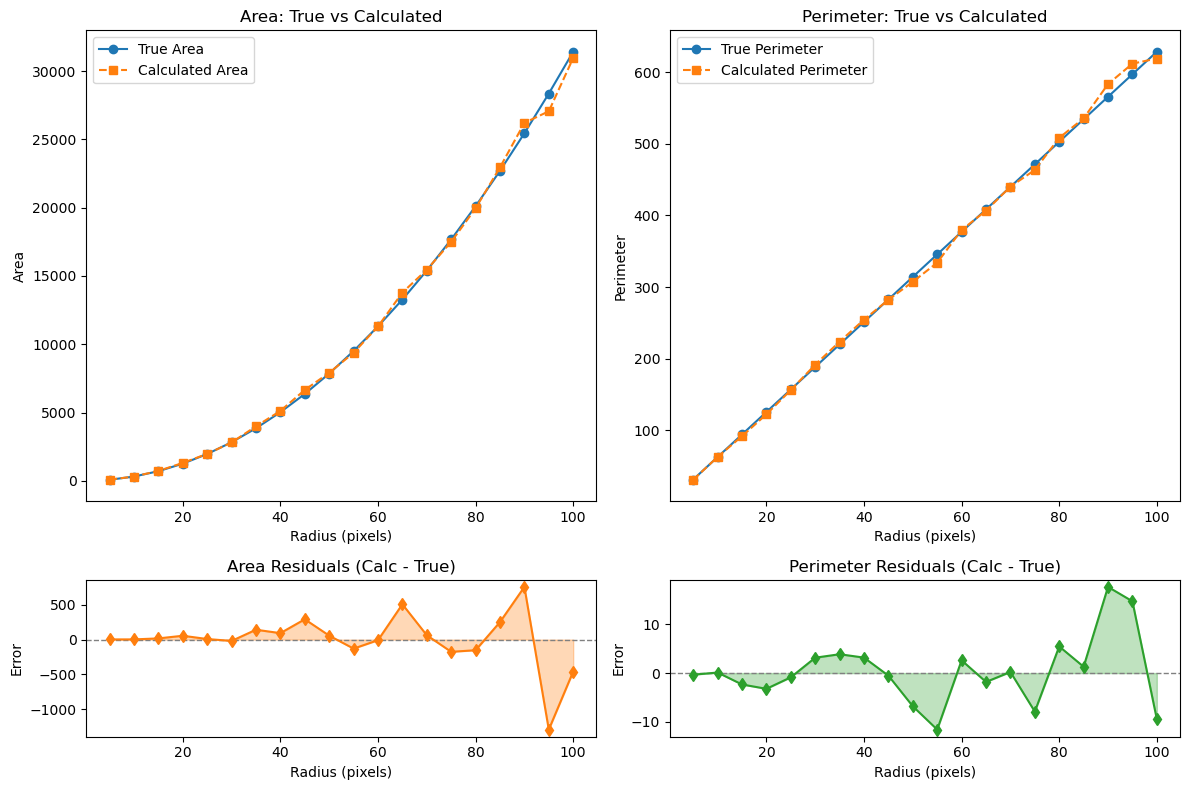
\includegraphics[width=0.75\textwidth]{figures/perimeter_area_uncertainties.png}
    \caption{Example of the uncertainty distributions in the measurements of perimeter and area from simulated structures (arbitrary units).}
    \label{fig:uncertainties}
\end{figure}
